\section{Echtzeitholographie}
\subsection{Versuchsbeschreibung}
Bei der Echtzeitholographie wird ein Hologramm aufgenommen und dieses mit dem Bild des Objektes überlagert. Unterschiede zwischen dem Objekt und seinem Hologramm können dann als Interferenzmuster beobachtet werden, solange sie nicht zu groß sind. In unserem Experiment wollen wir mit dieser Methode die resonanten Schwingungen einer fest eingespannten Aluminiumplatte untersuchen. Dazu nehmen wir zuerst ein Hologramm von dieser auf und entwickeln dieses. Mit einem Lautsprecher und einem Frequenzgenerator wird dann die Platte in Schwingung versetzt. Das Interferenzmuster erlaubt dann Rückschlüsse auf die Verformung und zeigt bei den Resonanzfrequenzen ein charakteristisches Muster.

\subsection{Durchführung und Auswertung}

Wir haben den Aufbau analog wie im vorherigen Versuchsteil verwendet. Anstelle der Stäbe haben wir allerdings die Aluminiumplatte eingebaut und den Lautsprecher hinter dieser plaziert. Da das Interferenzmuster Änderungen im Wellenlängenbereich anzeigt, sollte die Photoplatte nicht bewegt werden. Die Aufnahme und Entwicklung findet daher "`in-situ"' statt, d.h. in einem Tauchbecken am Ort der Aufnahme. Dazu werden anstelle der Planfilme nun Photoplatten, also Glasscheiben mit einseitig aufgetragener Photoemulsion, verwendet. Für deren Prozessierung haben wir wiederum mündlich überlieferte \cite{lena_christian} Prozessparameter verwendet:

\begin{table}
 \begin{tabular}{l}
  10 min quellen\\
  6 min belichten\\
  4 min entwickeln\\
  10 sec vorwässer\\
  2 min wässern\\
  1 min bleichen\\
  3 x 30 sec wässern\\
  1 min wässern\\
  volllaufen lassen
 \end{tabular}
 \caption{Prozessschritte für die Erstellung von Holographien auf Photoplatten}
\end{table}

Unsere erste Aufnahme ist eher als Probelauf zu verstehen, da wir das Prinzip der Fixierung der Glasplatten mit Metallklammern nicht verstanden hatten. Ursache dafür war vermutlich das sich diese nicht beim Tauchbecken befanden, sondern erst von uns gesucht werden mussten. Die resultierende Aufnahme zeigte dann nich einmal das ungestörte Hologramm (nur Referenzbeleuchtung). Die zweite Aufnahme, diesmal mit Befestigung, schien ebenfalls kein Hologramm ergeben zu haben. Als wir jedoch am nächsten Tag wiederkamen und den Laser einschalteten, konnten wir klar und deutlich ein Hologramm der Aluminiumplatte erkennen. Auch hatte die Flüssigkeit im Tauchbecken in der Zwischenzeit eine braune Färbung angenommen. Es ist also vermutlich Entwickler durch den leicht undichten Hahn nachgelaufen und hat für eine Nachentwicklung gesorgt. Das Hologramm ist in Abbildung \ref{hologramm_aluplatte} zu sehen. Wir haben dann versucht, Schwingungsresonanzen der Platte aufzunehmen, konnten diese aber nicht finden. Vermutlich waren Tauchbecken und Aluminiumplatte in der Zwischenzeit durch Erschütterungen oder versehentliches Anstoßen schon gegeneinander verrückt. Dafür spricht auch, das wir die sonst bei ausgeschaltetem Lautsprecher sichtbaren Interferenzmuster auch nicht sehen konnten.  

\begin{figure}[ht]
 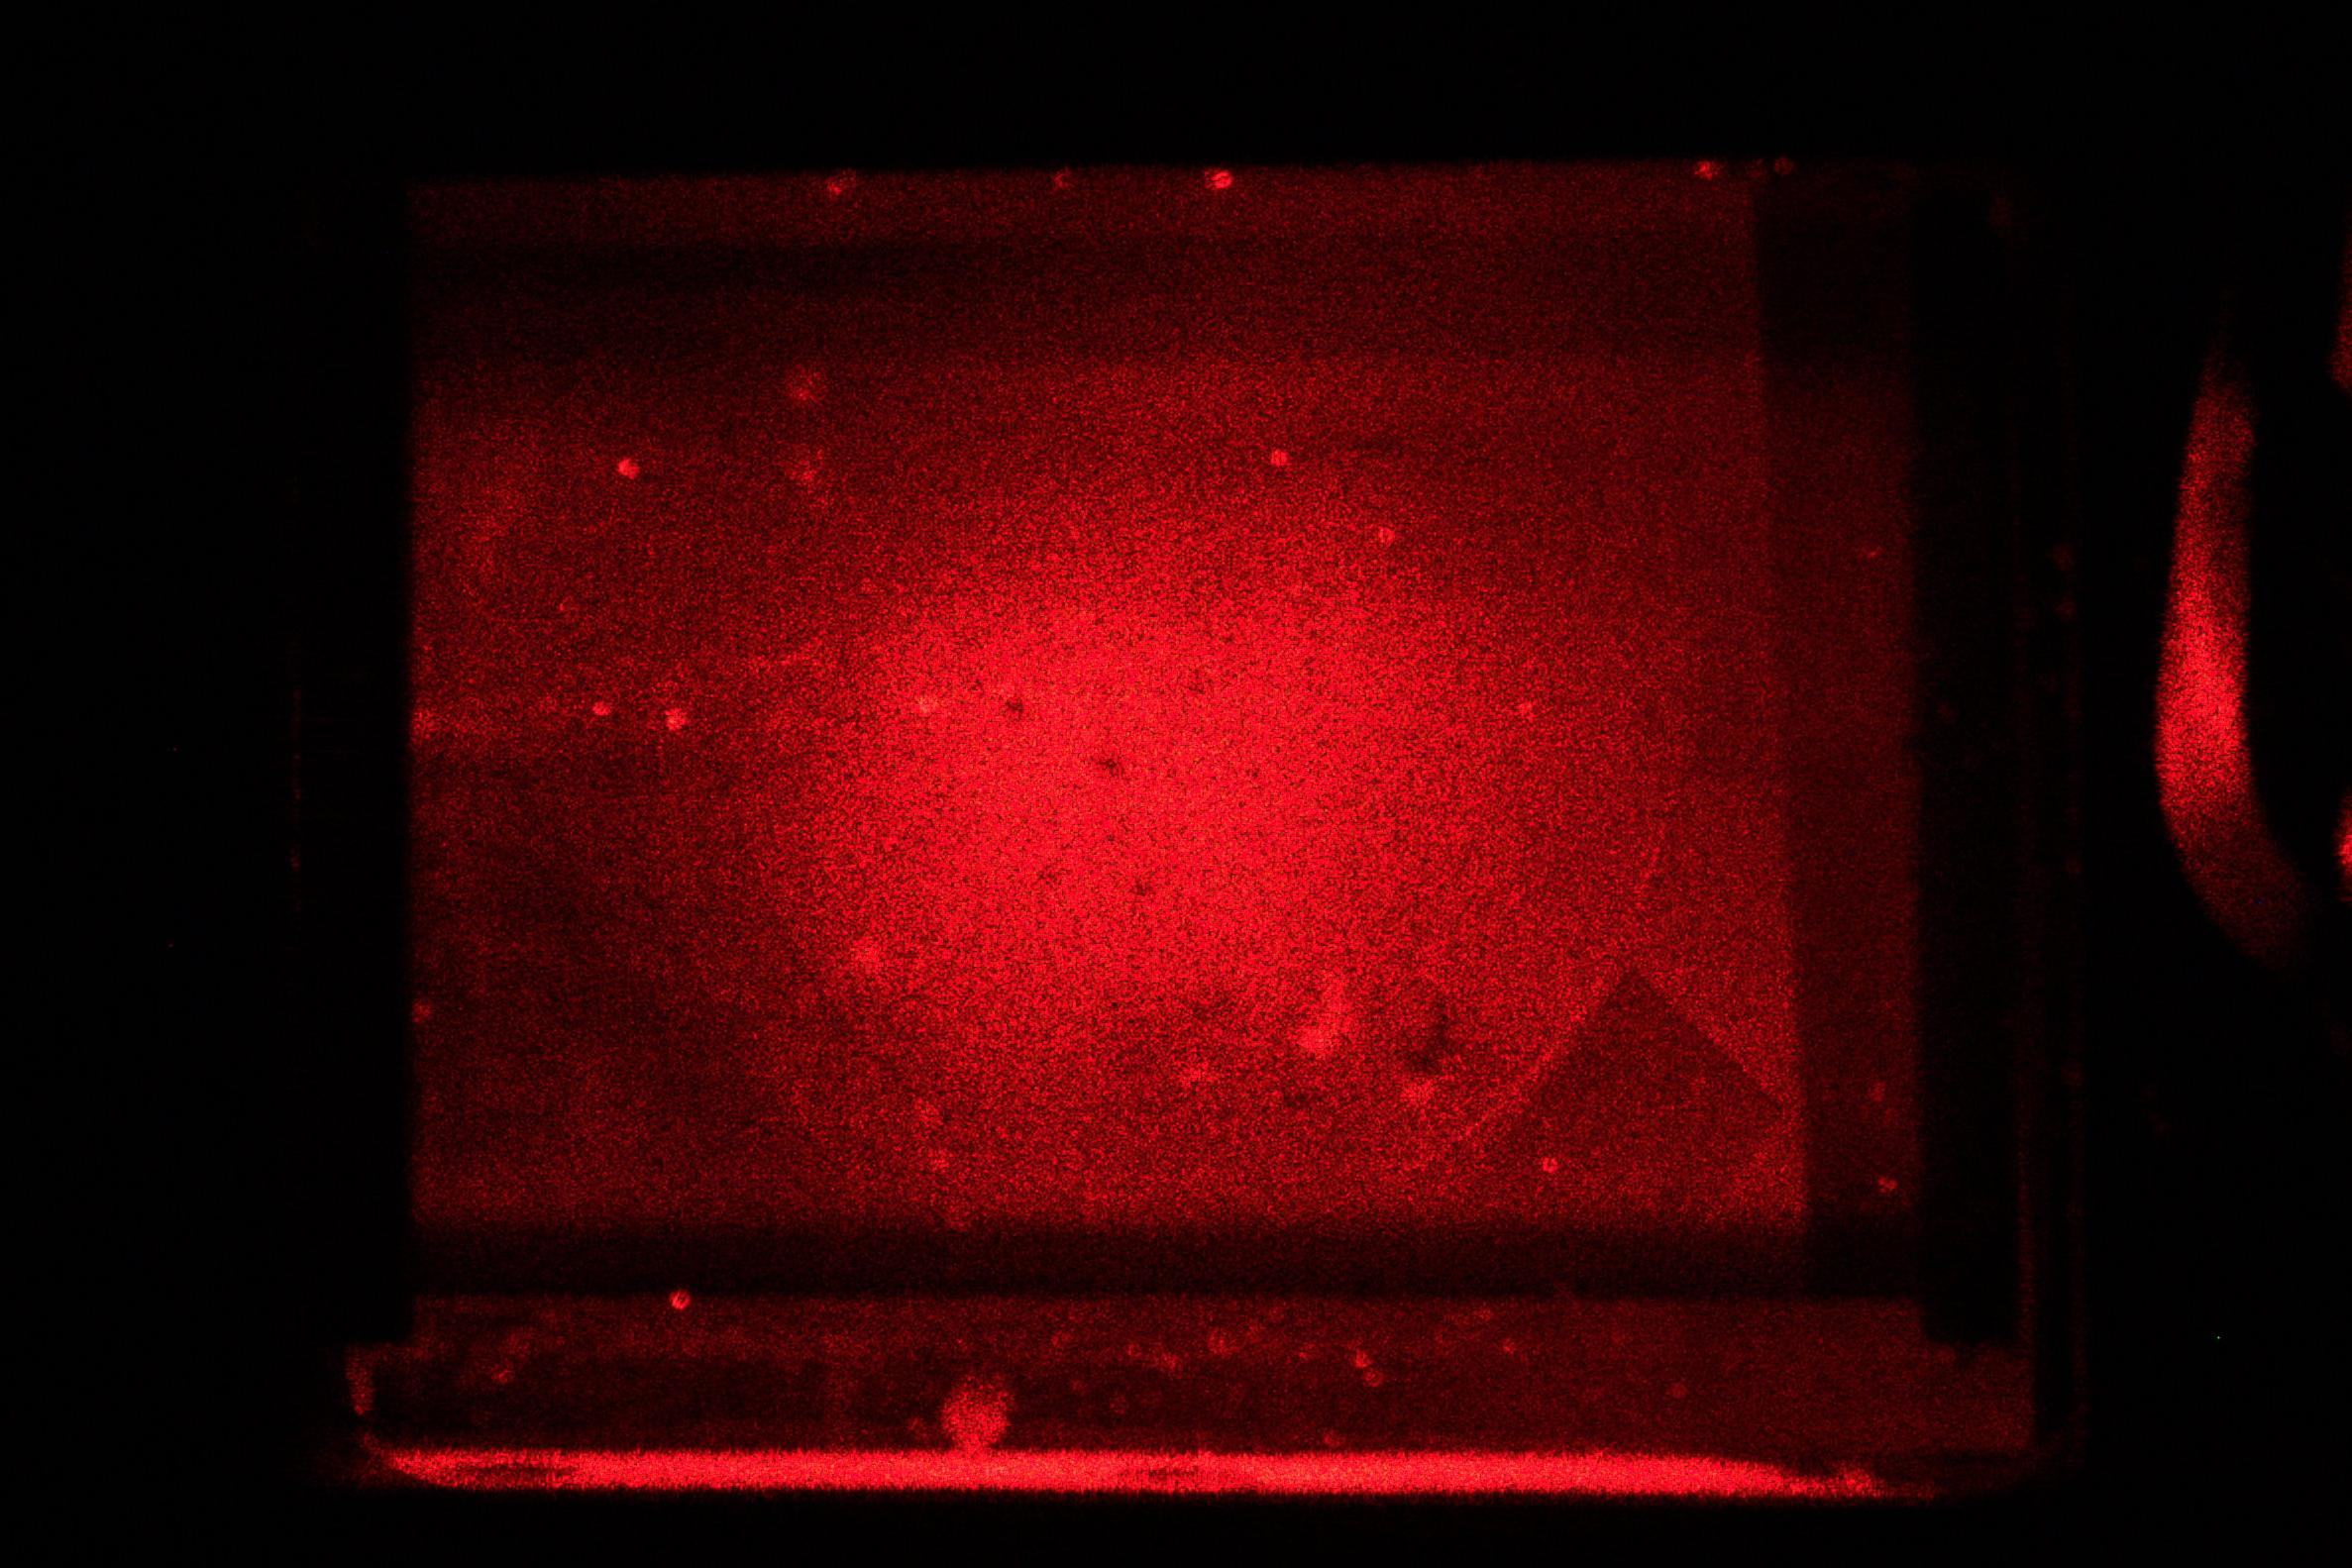
\includegraphics[width=\textwidth]{Photos/IMG_3927.jpg}
 \caption{Hologramm der Aluminiumplatte}
 \label{hologramm_aluplatte}
\end{figure}

Nach dieser Aufnahme war leider die Bleiche nahezu aufgebraucht. Auch Herr Stützler konnte uns keinen Nachschub liefern, da die Chemikalienausgabe in dieser Woche urlaubsbedingt vakant war. Seinen Vorschlag die Reste aus dem Auffangbehälter zu recyceln mussten wir leider ebenfalls verwerfen, da Geruchs- und Sichtproben uns deutliche Hinweise auf eine Verunreinigung mit Entwicklerlösung gaben. Wir haben daher die verbleibenden Reste im Zulauf im Verhältnis 1:7 mit Wasser gestreckt. Zusätzlich haben wir noch die (teilweise schon auskristallisierten) Reste aus dem Bleichebecken für die Filmentwicklung hinzugegeben. Eine verlängerte Bleichezeit von 5min gab uns bei der dritten Photoplatte zwar kein vollkommen gebleichtes Bild, kam dem aber sehr nahe. Mit diesem waren jetzt auch im ungestörten Zustand der Platte Interferenzmuster erkennbar, wie wir es erwartet hatten.

%TODO: BILD kein Ton (3932)

%TODO: BILD mit Ringen (3929-3931 481Hz) bzw. (3933-3934 482Hz)

Daher haben wir nun den Frequenzgenerator angeschaltet und versucht die Resonanzfrequenzen zu finden. Für die nullte Schwingungsmode ist uns dies auch gut gelungen. Bei einer Frequenz $f_{00} = 481 Hz$ %TODO: Abb
bzw $f_{00} = 482 Hz$ %TODO: Abb
konnten wir klar ein konzentrisches Kreismuster im Hologramm erkennen. Außerdem konnten wir dies auch akustisch anhand der resonanten Verstärkung bzw. der Schwebung bei geringfügiger Abweichung bestätigen. Das Muster war im Frequenzbereich von 478Hz bis 485Hz erkennbar. Die Lautstärke mussten wir dabei sehr gering wählen, an der Grenze der Hörschwelle, da die Minima sonst nur deutlich schwächer zu sehen wären. 